%\documentclass{mai_book}

%\defaultfontfeatures{Mapping=tex-text}
%\setmainfont{DejaVuSerif}
%\setdefaultlanguage{russian}
%\begin{document}
\cleartop

\hspace{3.4in}АЛГЕБРАИЧЕСКАЯ

\hspace{3.4in}АЛГОРИТМИКА
\newpage
\hspace{3.0in} LOGIQUE MATHEMATIQUES

 \hspace{3.1in} \textbf{I N F O R M A T I Q U E}
\\\\\\
{\Huge \textbf {ALGORITMIQUE}}
\\
\newline {\Huge \textbf {ALGEBRIQUE}}
\\\\
\Large{ \textbf{Avec exercices corriges}}
\\\\\\\\\\
\normalsize {Patrice NAUDIN}
\newline \textit {\normalsize {Maitre de conferences a I'universite de Bordeaux I}}
\\\\
\normalsize {Claude QUITTE}
\newline \textit {Maitre de conferences a I'universite de Poitiers}
\\\\
\normalsize {Preface de Francis SERGERAERT}
\\\\\\\\\\\\\\\\\\\\\\\\\\\\\\\\\\\\\\\\\

\hspace{2.0in} MASSON Paris Milan Barcelone Bonn 1992
\newpage
\large {Патрис НОДЕН},    \large {Клод КИТТЕ}
\\\\\\\
{\Huge \textbf {АЛГЕБРАИЧЕСКАЯ}}
\\
\newline {\Huge \textbf {АЛГОРИТМИКА}}
\\\\\
\textbf{С упражнениями и решениями}
\\\\\\
\newline Предисловие Франсиса Сержераера
\\\\\\\
Перевод с французского
\newline \textit{В.А. Соколова}
\\\\
под редакцией
\newline \textit {Л.С. Казарина}
\\\\\\\\\
\small {Рекомендовано Научно-методическим советом по прикладной математике
\newline Учебно-методического объединения университетов для использования в учеб-
\newline ном процессе для студентов вузов по специальности «Прикладная математи-
\newline ка» и «Прикладная математика и информатика»}
\\\\\\\\\\\\\\\\\\\\\\\\

\includegraphics{2.png}

\large {МОСКВА «МИР» 1999}
\newpage

УДК 512+519.6

   ББК 22.14+22.19

\hspace{1.0cm} Н72
\\

\hspace{1.0cm} \textbf{Ноден П., Китте К.}

Н72 \hspace{0.5cm} \small {Алгебраическая алгоритмика (с упражнениями и решениями):} 

\hspace{1.0cm} \small {Пер. с франц. — М.: Мир, 1999. — 720 с., ил.}

\hspace{1.5cm} ISBN 5-03-003318-1

\hspace{1.5cm} \small {Книга известных французских математиков — это по существу эн-

\hspace{1.0cm} циклопедия алгоритмов алгебры и теории чисел от Евклида и до на-

\hspace{1.0cm} ших дней. В ней прослеживается общая идея — представить основные

\hspace{1.0cm} алгебраические структуры и концепции в виде объектов, поддающих-

\hspace{1.0cm} ся машинной обработке. Главными для авторов являются два вопроса:

\hspace{1.0cm} что значит вычислить математический объект и как его вычислить

\hspace{1.0cm} наиболее эффективно.

\hspace{1.5cm} Изложение отличается методическими достоинствами: тщательный 

\hspace{1.0cm} отбор материала, многочисленные замечания теоретического и исто-

\hspace{1.0cm} рического характера, большое число упражнений с решениями в конце

\hspace{1.0cm} каждой главы.

\hspace{1.5cm} Для математиков-прикладников, для всех изучающих и применяю-

\hspace{1.0cm} щих компьютерную алгебру и информатику как учебное и справочное 

\hspace{1.0cm} пособие.}

\hspace{4.0in} ББК 22.14+22.19
\\

\hspace{2.4in} 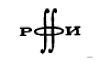
\includegraphics{1.png}
\\

\hspace{2.0cm} Издание осуществлено при поддержке Российского фонда 

\hspace{2.3cm}фундаментальных исследований по проекту 97-01-14001
\\\\

\hspace{2.5cm} Издание осуществлено в рамках программы помощи 

\hspace{2.9cm} издательскому делу «Пушкин» при поддержке 

\hspace{3.2cm} Министерства Иностранных Дел Франции

\hspace{4.0cm} и Посольства Франции в России
\\\\
 
\hspace{2.0cm} \textit {Редакция литературы по математическим наукам}
\\\\

ISBN 5-03-003318-1 (русск.) \hspace{2.1cm} © Masson, Paris, 1992 

 ISBN 2-225-82703-6 (франц.) \hspace{2.0cm} © перевод на русский язык,
 
\hspace{2.8in} «Мир», 1999
\newpage
\vspace*{50pt}
\hspace{2.0cm} {\Large \textbf {Предисловие переводчика}

\hspace{2.6cm} {\Large \textbf {и редактора перевода}.
\\\\

\noindent\normalsize {Со времени появления монографии Г. Биркгофа и Т. Барти «\textit {Современ-\linebreak ная прикладная алгебра}» (28 лет тому назад) сочетание прилагатель-\linebreak ных «\textit {прикладной}» и «\textit {абстрактный}» в применении к алгебре перестало\linebreak  шокировать или изумлять читателей. Прилагательное «\textit {современный}»,\linebreak разумеется, должно исчезнуть по мере разрастания теории и завоева-\linebreak ния все новых территорий (переведенная недавно книга Р. Лидла и\linebreak П. Пильца тому свидетельство). Более интересным является сопоста-\linebreak вление компьютерной математики и алгебры, появившееся сравнитель-\linebreak но недавно, а уж алгебраическая алгоритмика и вовсе должна вызвать\linebreak ассоциацию с «\textit {маслом масляным}», ибо корни обоих понятий (алгебра и\linebreak алгоритм), как известно, одни и те же. Тем не менее, несмотря на близ-\linebreak кое родство, алгоритмика (читай, информатика) и алгебра длительное\linebreak время развивались как бы обособленно, хотя слово «\textit {метод}» в учебни-\linebreak ках по высшей алгебре вытеснялось постепенно словом «\textit {алгоритм}», а\linebreak в информатику проникли модули и тензорные произведения. Вопросы\linebreak сложности вычислений, явившиеся краеугольным камнем для информа-\linebreak тики, позволили поставить весьма интересные чисто алгебраические\linebreak задачи. Стало ясно, что в алгебре можно вычислять, даже если исход-\linebreak ные вопросы касаются таких субстанций, как модуль, кольцо, группа.\linebreak А раз можно вычислять, то нужно вычислять как можно быстрее, ибо\linebreak уже студенту-первокурснику понятно, что «\textit грубая сила» машины не\linebreak сможет выручить при решении некоторых совсем простых, на первый\linebreak взгляд, задач.
    
   Многие алгоритмы алгебры, с которыми нам приходилось сталки-\linebreak ваться в жизни, становились известными из математического фольк-\linebreak лора, другие изобретались самостоятельно (ибо посмотреть было не-\linebreak где). Потом появился изумительный Д. Кнут (Искусство программиро-\linebreak вания), пугающий своей фундаментальностью, куда все-таки приходи-\linebreak лось заглядывать, невзирая на известные трудности. А что делать сту-\linebreak денту? Книга «\textit {Алгебраическая алгоритмика}» явилась нам неожиданно\linebreak во всем своем блеске благодаря знакомству с ее авторами, работавши-\linebreak ми в Пуатье. Начав работать, мы оба поняли, что этой-то книги нам\linebreak не хватало и как преподавателям, и как математикам-профессионалам.}
   
\newpage 
\restoretop
\newtoplo{Предисловие переводчика и редактора перевода}
\newtopre{Предисловие переводчика и редактора перевода}
\setcounter{page}{6}% ВОТ ТУТ ЗАДАТЬ СТРАНИЦУ
\noindent
С одной стороны, — это новый взгляд на вещи, казавшиеся устоявшимися. Например, что может быть проще алгоритма Евклида или возведения в степень? С другой, некоторая систематизация, азбука информатики (как мы мечтали 30 лет тому назад о каталоге полиномиальных алгоритмов!). Наконец, это философия программирования, изложенная на небольшом пространстве и без присущего сугубым профессионалам высокомерия.

В то же время книга читается (мы отмечаем это с некоторым ужасом) как художественная, беллетристическая литература. Чего стоит одно дерево Штерна — Броко из задачи 35 в главе II!

   Основной материал книги сопровождается огромным количеством упражнений (их около 300, но некоторые из упражнений содержат в себе от 3 до 5 задач), примеров, иллюстраций. Студента несомненно порадует то обстоятельство, что большинство упражнений приводится с решением (не сразу, а через несколько страниц). Пересечение с другими известными нам книгами по алгоритмике невелико.
   
Книга П. Нодена и К. Китте восполняет пробел, существовавший в литературе на русском языке (и по математике, и по информатике), и может быть использована для чтения специальных и основных курсов как для студентов-математиков, так и для информатиков. Кроме того, она, будучи использована в качестве дополнительного источника, окажется несомненно полезной при чтении курсов «Алгебра и теория чисел» и «Алгебра и геометрия».

   Следует отметить, что терминология, применяемая французскими математиками, не вполне совпадает с принятой в нашей литературе. Так, натуральный ряд начинается с нуля, а не с 1, как обычно принято у нас. Отсюда появление обозначения N*. Приведение матрицы к ступенчатому виду осуществляется по столбцам, а не по строкам, причем имени Гаусса авторы в этой связи не упоминают. Есть и другие мелкие детали, которые читатели, несомненно, заметят. Что ж, это заставляет читателя быть внимательным!

  Приятно отметить, что в подготовке к изданию перевода книги активное участие приняли наши ученики и студенты С.В. Монахов, С.М. Медведев (подготовившие оригинал-макет русского перевода), И.А. Сагиров, Л.В. Гудкова, А.В. Хлямков, А.Е. Скрипкин. Мы им выражаем нашу глубокую благодарность. Мы также признательны заведующему лабораторией теоретико-групповых методов профессору А.Л. Онищику за предоставление технических средств для верстки этой книги. Мы благодарны издательству MASSON, давшему согласие на передачу права на издание перевода книги издательству «Мир», и Посольству Франции в Москве включение русского издания книги
\pagebreak
в программу «Пушкин», а также Российскому фонду фундаментальных исследований, поддержавшему проект перевода книги издательским грантом.

   В заключение мы хотим прямо сказать, что наш замысел вряд ли осуществился, если бы не помощь и активное сотрудничество наших французских друзей и коллег из университета Пуатье — авторов книги Патриса Нодена и Клода Китте. Они дали согласие на безвозмездное издание перевода их книги, любезно предоставили в наше распоряжение файлы с ее электронным вариантом и постоянно, на протяжении всего времени работы над переводом, поддерживали с нами связь, консультировали нас, полностью пересмотрели текст французского издания и внесли в него много исправлений и улучшений, которые учтены в русском издании.
   
   Только благодаря этому сотрудничеству наш совместный проект успешно завершен.
   
   Надеемся, что перевод этой примечательной книги будет интересен и полезен нашим читателям.


 \hspace{3.1in} \textit {Л.С. Казарин, В.А. Соколов,} 
   
\hspace{3.0in} \textit {Ярославль, 10 августа 1998 г.}
\newpage
\cleartop
\vspace*{50pt}
\hspace{1.4cm} {\Large \textbf {Предисловие к русскому изданию}}
\newline\\
\hspace*{15pt}
\hspace*{15pt}
\\\\
Проект перевода Львом Казариным и Валерием Соколовым нашей кни-
ги «Алгебраическая алгоритмика», возникший более двух лет тому на-
зад, подошел к завершению. Мы особенно рады этому событию, ес-
ли учесть, что пройденный путь, вероятно, не был гладким. Основные очертания проект приобрел в результате нашего путешествия в Россию, которое мы предприняли весной 1996 года по приглашению Валерия Соколова от имени Ярославского государственного университета. Во время нашего пребывания в Ярославле Лев и Валерий оказали нам, как гостям университета, самый радушный прием. Лев сопровождал нас во всех поездках, которые Ярославский университет организовал для нас, чтобы мы открыли для себя маленький кусочек России — это то, что выходит за рамки профессиональной деятельности, но является, тем не менее, приятным (и необходимым) элементом любой поездки за границу. Благодаря Льву мы открыли ряд исторических уголков, входящих в «Золотое кольцо»; он опекал нас на первых шагах в нашей повседневной жизни иностранцев в России, что порой было очень непросто: вспомним автобус, который отвозил нас на вокзал в пятницу в 6 часов утра, когда все киоски были еще закрыты! «Автобус... А как насчет билетов?» А в Москве Аркадий Онищик, Сергей и Ирина Струнковы доказали нам на непостижимом для представителей Запада уровне, что российское гостеприимство вовсе не легенда. Обо всех этих встречах и людях мы сохраним самые волнующие воспоминания.

   Прервем здесь дифирамбы, хотя это вступление в действительности лишь в небольшой степени передает наше душевное состояние. Нелегкое, все-таки, это дело — сочинять предисловие к переводу книги, которую сами написали! Поговорим, однако, об идеях, которые мы хотели изложить в этой книге.

   В течение трех лет работы над ней (1989-91 гг.) нашей целью — амбициозной и одновременно наивной — было представить с одной конкретной точки зрения некоторые разделы алгебры, преподаваемые на старших курсах университета. В то время нам хотелось (и сейчас нам этого хочется более, чем когда-либо) изменений в изложении математики: не отказываясь от абстрактных понятий, использовать их так, чтобы гармонично сочетать теорию и практику.
   
\pagebreak
\restoretop
\newtopre{Предисловие к русскому изданию}
\newtoplo{Предисловие к русскому изданию}
   Любой студент-математик знаком с основными понятиями, которые\linebreak
встречаются в арифметике: целые числа, сравнимость чисел по моду-\linebreak
лю $n$, многочлены и т.д. Но, чаще всего, эти объекты, по самой своей\linebreak
сути предназначенные для практики, определяются очень формально\linebreak
и абстрактно. Так ли уж необходимо вводить фактор-группу некото-\linebreak
рой группы по отличной от нее подгруппе для изучения целых чисел,\linebreak
сравнимых по модулю п? Что усвоят наши студенты при таком подхо-\linebreak
де? Так ли уж неразумно опираться, когда это возможно, на практику?\linebreak
Ведь освоив вычисления по модулю целого числа (или по модулю мно-\linebreak
гочлена), уже гораздо позже можно рассмотреть общий случай вычи-\linebreak
слений по модулю идеала, «более естественно» приводящий к понятию\linebreak
фактор-кольца. В самом деле, нет недостатка в конкретных проблемах,\linebreak
где может с успехом использоваться вычислительная практика: тест на\linebreak
простоту чисел Лукаса — Лемера, критерий Пепина, RSA-метод в кри-\linebreak
птографии, генератор случайных чисел и т.д. Мы рассматриваем все\linebreak
эти темы в нашей книге и убеждены, что они лучше подходят для обу-\linebreak
чения, чем «теорема о факторизации (переход к фактор-множеству)\linebreak
некоторого отображения».

   Что же изменилось с 1992 года, времени выхода нашей книги? В\linebreak
области математической алгоритмики на рынке появилось некоторое\linebreak
количество монографий, но это в основном узко специализированные\linebreak
книги научного характера, оказывающие весьма слабое влияние на пре-\linebreak
подавание математики. Что же касается информатики как таковой,\linebreak
то единственным плодом ее непрерывного бурного развития в дан-\linebreak
ной области является увеличение числа систем формальных вычисле-\linebreak
ний — часто настолько же мощных, насколько и непоследовательных,\linebreak неприспособленных для научной работы из-за недостаточной строго-\linebreak
сти. Нынче можно осуществлять сложные вычисления в теории Галуа, в\linebreak алгебраической геометрии, в теории чисел, в теории групп и т.д., но все\linebreak
это, как правило, недоступно для начинающего студента-математика.\linebreak
И против всех ожиданий, области, в которых системы формальных вы-\linebreak
числений уже хорошо обкатаны — это, как ни странно, разделы курса\linebreak
алгебры — всегда излагаются в том же виде, в каком они были де-\linebreak
сятилетия назад. Использование этих прикладных программ осталось\linebreak
вне преподавания математики и касается, в основном, лишь научных\linebreak
исследований.

   Сообществу математиков, кажется, грозит опасность раскола на\linebreak
два чуждых друг другу мира: «теоретиков» и «алгоритмистов». Эта
\linebreak
ситуация, на наш взгляд, была бы достойна сожаления. В то же время,\linebreak
во Франции — особенно в преподавании математики — нередко шли\linebreak
на отказ от догматических воззрений в пользу нового хорошего подхо-\linebreak

\pagebreak
\noindent
да к объяснению того или иного понятия. Преподавание (равно, как и научное исследование) может лишь обогатиться благодаря многообразию способов изложения материала: достаточно хотя бы раз в жизни прочитать студентам курс лекций по алгоритмике, чтобы убедиться в этом.

\hspace{3.8in} П. Ноден, К. Китте,
        
\hspace{3.3in} Пуатье, 2 февраля 1999 г.
\newpage
\cleartop
\vspace*{30pt}
\begin{center}
\textbf{\Large Предисловие}
\end{center}
   Патрис Ноден и Клод Китте попросили меня написать предисловие к их книге, и я начну с благодарности им: быть вовлеченным в работу в приятной компании по случаю выхода в свет такого прекрасного произведения — это счастье.

   История математики очень увлекательна. Для сюжета, который нас занимает сегодня, существенны три персонажа. Евклид пишет свои «Начала» за три столетия до нашей эры, и с этой даты большинство историков ведут отсчет появления той математики, которую мы знаем сегодня, имеющей характер некой игры, заключающейся в том, чтобы делать интересные выводы из множества хорошо подобранных аксиом. Природа этих аксиом и соблюдаемые правила игры с самого начала не были достаточно ясны, и математика XIX века познала такое развитие, что вскоре основы здания были едва способны выдерживать всю конструкцию. Итогом этого было то, что называют кризисом оснований математики.

   Но тут появился Гильберт; он понял и талантливо объяснил, что математика может быть формализована. Гильберт описал работу математиков, как чисто формальную игру, манипулирующую множеством аксиом (комбинаторных объектов) с помощью доказательств (чисто комбинаторной техники) и приводящую к теоремам (также комбинаторным объектам). На самом деле так говорить — неправильно: Гильберт мог таким образом описать результаты, полученные его предшественниками, но никоим образом — с помощью какой процедуры они их открыли. Это главное различие для того сюжета, которым мы интересуемся. Гильберт знал это и вскоре поставил перед сообществом хорошие вопросы на эту тему: может ли аксиоматическая система быть полной, или, другими словами, всякое ли утверждение, имеющее смысл в этой системе, истинно или ложно? Кроме того, существует ли алгоритм, позволяющий определять, истинно или ложно то или иное утверждение (или же невыводимо в случае неполноты)?

   После Евклида и Гильберта третьим является Гёдель. Он доказал,\linebreak
что всякая аксиоматическая достаточно «интересная» теория обяза-\linebreak
тельно будет неполной (или противоречивой). Этот явно негативный\linebreak
результат странным образом является одним из наиболее позитивных.\linebreak
   
\pagebreak
\restoretop
\newtopre{Предисловие}
\newtoplo{Предисловие}
\noindent
Непосредственно вдохновленные доказательством Гёделя логики Чёрч\linebreak
и Тьюринг вскоре доказали (1936), независимо друг от друга и разными\linebreak способами, что второй вопрос Гильберта также имеет отрицательный\linebreak
ответ: не может существовать алгоритм, даже чисто теоретический,\linebreak
грозящий математикам безработицей. Этот результат все еще отри-\linebreak
цательный, но — терпение, и мы увидим, что на самом деле Чёрч и\linebreak
Тьюринг стоят у истоков фантастической — и позитивной — револю-\linebreak
ции в математике. Ибо им пришлось очень тщательно обдумать, что\linebreak
же такое алгоритм. Первый из них изобрел для уточнения этого поня-\linebreak
тия A-исчисление, второй — свою знаменитую теоретическую машину.\linebreak
И это стало рождением целой новой ветви в математике, называемой\linebreak
алгоритмикой, и книга, которую я предваряю предисловием, частично\linebreak
относится к этой области. В этом ее новизна.

   Благодаря фон Нейману идеи Тьюринга вскоре привели к концеп-\linebreak
ции и реализации того, что теперь называется компьютерами. Вначале\linebreak
в них видели лишь инструмент, предназначенный для того, чтобы ис-\linebreak
пользовать результаты труда математиков-теоретиков в различных\linebreak
приложениях. Этот взгляд, все еще распространенный, когда инфор-\linebreak
матик ниже по течению принимает эстафету от математика, является\linebreak
сегодня совершенно неверным. Больше уже не считают, что матема-\linebreak
тические теории, представление о которых существенно изменилось,\linebreak
находятся в верховьях по отношению к положению алгоритмического\linebreak
инструмента, и ставить эту ветвь в подчинение другим так же наив-\linebreak
но, как пытаться выяснить в алгебраической топологии, что главнее:\linebreak
топология по отношению к алгебре или наоборот.

   Математики все еще часто и довольно нелепо считают за честь полу-\linebreak
чить результаты, не использующие новые алгоритмические средства.\linebreak
Это обычное явление, сопровождающее значительное и быстрое раз-\linebreak
витие в какой бы то ни было сфере жизни: подобное развитие поро-\linebreak
ждает кризис, разрешающийся более или менее удачно. Когда возникла\linebreak алгебраическая топология, многие строптивые топологи старательно\linebreak
отделяли топологические доказательства, не использующие алгебраи-\linebreak
ческую топологию, считая их более хорошими, от других, незаконно-\linebreak
рожденных. Но в конце концов алгебраическая топология утвердилась.\linebreak
В рамках алгебраической топологии в один прекрасный день появи-\linebreak
лись спектральные последовательности', в это время доказательства,\linebreak
использующие такую технику, еще рассматривались как «грязные», и\linebreak
их, по-возможности, избегали. Мало-помалу, спектральные последова-\linebreak
тельности стали обычным делом. Совсем недавно новые исследования\linebreak
заново изучили вопрос, связанный со спектральными последовательно-\linebreak
стями, для того, чтобы сделать из них алгоритмический инструмент;\linebreak

\pagebreak
\noindent
я знал редактора одного прекрасного математического журнала, сердито требовавшего представить аргумент, «убеждающий», что новые результаты, полученные таким способом, были бы недоступны при использовании «других средств» (sic) и не иначе, без чего представленная статья на эту тему была бы, очевидно, отвергнута. S.O.S. — расизм!

   Книга Патриса Нодена и Клода Китте представляет классическую алгебру — ту, которая преподается на уровне второго цикла университета, но в свете новой алгоритмической идеологии. Для рассматриваемой темы алгебра подходит лучше всего: алгоритмика по самой своей природе комбинаторна, а среди всех основных математических дисциплин алгебра является, несомненно, «самой комбинаторной». Преподавать студентам алгебру таким способом — прекрасная идея с разных точек зрения. Очень полезно, что значительно усиливается конкретный характер теории, результатов, упражнений, отдельных тем; это облегчает понимание, требует хорошей точности, но и придает характер игры занятию, которое нередко воспринимается скучным и отталкивающим.

   Но есть еще более важное обстоятельство. Богатство, присущее математике, чаще всего требует, как, впрочем, и в любой сфере деятельности, использования сразу нескольких средств очень разной природы. Самые большие успехи в математике почти всегда могут быть описаны именно так. В другой области, теоретической физике, показательна работа Луи де Бройля, объясняющая, что правильно понять свойства материи можно, лишь рассматривая ее одновременно с волновой и корпускулярной точек зрения. Эйнштейн поступил аналогично в отношении массы и энергии, Гильберт — с геометрией и функциональным анализом и т.д. Так и с момента возникновения алгоритмики всякая попытка пересмотреть тот или иной раздел математики с точки зрения алгоритмики может быть встречена с интересом и надеждой.

   Так устанавливаются взаимные связи, природа которых богата и\linebreak
разнообразна. В некоторых случаях алгоритмика оказывается на служ-\linebreak
бе у обычной математики, являясь тогда инструментом прикладной ма-\linebreak
тематики. Часто использование средств алгоритмики порождает но-\linebreak
вые области математических исследований. Проблемы сложности вы-\linebreak
числений, составляющие значительную часть данного труда, — это как\linebreak
раз тот самый случай. Замечу, кстати, что именно к этой области при-\linebreak
надлежит самая важная открытая проблема современной математики\linebreak
— сравнение сложностей Р и NP; если, основываясь на сравнительном\linebreak
подобии, распространить математику на все науки, то проблемы Рима-\linebreak
на, Пуанкаре, «обратная теорема Галуа» окажутся где-то недалеко от\linebreak
химии, тогда как проблема $P \neq N P$ не выйдет за пределы математики.\linebreak

\pagebreak
   Иной раз алгоритмические проблемы порождают новый сюжет, ко-\linebreak
торый может быть затем полностью отделен от источника своего про-\linebreak
исхождения и превратиться в раздел «чистой» математики. Хоть исто-\linebreak
рически это и не вполне корректно, но таким образом можно пред-\linebreak
ставлять студентам гармонический анализ. Одна из глав этой книги\linebreak
посвящена дискретному преобразованию Фурье. Даже если бы Фурье\linebreak
не существовал и даже если бы никто с тех пор не мог его заменить,\linebreak
все равно алгоритмика умножения многочленов обязывает обнаружить\linebreak
так называемый анализ Фурье, его интерес, его богатство и его эф-\linebreak
фективность. А потом уже нетрудно, переходя к пределу, получить\linebreak
ряды Фурье и преобразование Фурье, исходя из дискретного преобра-\linebreak
зования Фурье; наиболее просто это сделать, используя нестандартный\linebreak
анализ — но берегись инквизиторов: сочетая две ереси в одном курсе,\linebreak
рискуешь сломать себе шею, если не быть осторожным или попросту\linebreak
скромным!

  Другой интересный случай, представляющий, несомненно, очень бо-\linebreak
гатый сюжет: для некоторой ранее существовавшей математической\linebreak
теории ее пересмотр может привести к таким точкам зрения, кото-\linebreak
рые требуют иных методов, имеющих свой собственный интерес, не\linebreak
уменьшая, однако, тем самым, интерес к исходным теоретическим ме-\linebreak
тодам. Хорошим примером такого сорта является матричное исчисле-\linebreak
ние. Классическая теория определителей, на базе знакопеременных по-\linebreak
лилинейных форм, непосредственно не используется при вычислении\linebreak
определителей. На самом деле ситуация даже еще лучше. Наши самые\linebreak
далекие предшественники, несомненно, были знакомы с сущностью так\linebreak
называемого метода Гаусса решения систем линейных уравнений. Од-\linebreak
нажды появились теоретики и вообразили, что лучше это делать с по-\linebreak
мощью определителей. Потом алгоритмисты снова поправили стрелки\linebreak
часов: для машины метод Гаусса намного лучше, чем метод Крамера,\linebreak
что, однако, вовсе не лишает интереса к этому методу, который с успе-\linebreak
хом используется для теоретического анализа первого. Этот и другие\linebreak
связанные с ним вопросы изящно изложены в данной книге; содержаща-\linebreak
яся в ней обширная библиография и комментарии позволят прилежным\linebreak
читателям быстро добраться до современных проблем, о богатстве ко-\linebreak
торых они вначале и не подозревали.

   Информатики сразу распознают одного из духовных наставников\linebreak
авторов: Дона Кнута. Отметим лишь составление макета книги, пол-\linebreak
ностью реализованное самими авторами (без Postscript’а!) с помощью\linebreak
TEX'a. Мне не известна официальная градация в сообществе TEX пер-\linebreak
тов, но, несомненно, Патрис Ноден и Клод Китте в его первом эшелоне.\linebreak

\pagebreak
   Вошло в поговорку безграничное богатство анализа всех аспектов проблемы в книгах Кнута; то же самое мы обнаруживаем здесь. Для читателя, раполагающего достаточным временем, эта книга — неисчерпаемый кладезь возможностей рассматривать отдельную тему с множества точек зрения. Когда, говоря о программе, авторы решаются перейти к следующей теме, они не забывают заранее указать полезную библиографию; часто это даже библиография в квадрате, содержащая цитируемые тексты, которые, в свою очередь, также содержат обширную библиографию — изящный пример использования подпрограмм. Как и у Кнута, в этой книге имеется обширный набор упражнений разного уровня — от простых примеров, предназначенных проверить понимание того или иного понятия, до самых сложных задач, приближающихся к темам научных исследований. И, как и у Кнута, решения упражнений также включены в книгу!

  Для изучения алгоритмов требовалась техническая поддержка в виде языковых средств информатики. Авторы выбрали язык Ада — безусловно, один из лучших на сегодня языков. И пусть потенциальные пользователи не волнуются по поводу выбора языка, все еще не слишком распространенного во французских университетах: перевод Ада- программ в их любимый язык является несложным техническим упражнением; при этом строгость документации программ просто поразительна и может служить примером, так что на этот счет нет никаких опасений. Такой перевод, требующий ясно отличать алгоритмическую часть от реализации, очень поучителен. Кроме того, авторы зачастую предварительно дают описание алгоритмов в чистом виде в соответствии с аксиоматикой Хоара.

   Это превосходная книга, которую я ставлю в моей библиотеке на полку со «священными» книгами, где находятся уже два «евангелия» — алгоритмика по Вирту и алгоритмика по Кнуту. Теперь я обладаю третьим «евангелием»; кто же напишет четвертое? Но ведь эта книга потребовала коллективной работы двух авторов — еще одно примечательное свойство, так что может быть моя коллекция «евангелий» уже полна? Нет: это противоречило бы Гёделю, но это уже совсем другая история.
   
\hspace{3.6in} Франсис Сержераер,

\hspace{3.1in} Мейлан, 27 сентября 1991 г.
\newpage
\cleartop
\vspace*{50pt}
\hspace{1.5in} \textbf{\Large От авторов}
\\\\\\\\
   Вот и наступил момент, когда, закончив книгу, автор начинает свое введение и ищет подходящие формулировки, которые убедили бы читателя, что все дальнейшее было спланировано, обосновано... с самого начала. Мы не будем отступать от этого правила. Однако, скажем откровенно, наша точка зрения изменялась многократно с того момента, когда мы принялись за этот труд.

   Вопрос «Возможно ли вычислять математические объекты?» является лейтмотивом этой работы; как можно убедиться, эта книга не дает окончательного ответа, но, надеемся, показывает, что этот вопрос не лишен интереса. В особенности в той области, которую затрагиваем здесь, а именно, в алгебре, мы убеждены, эффективное вычисление объектов — вручную или с помощью компьютера — проливает свет на используемые понятия. Но, начиная с таких элементарных понятий, как кольцо целых чисел по модулю п, и до более абстрактных структур, как модули в основных кольцах, что же все-таки можно вычислять и как? В начале работы мы были совсем уже готовы уступить намерению рассматривать алгебру без каких бы то ни было формальных средств, а только в чисто вычислительном аспекте; но изучение преобразования Фурье — и, в особенности, работы Ш. Винограда — убедительно подтолкнули нас к тому, чтобы избежать этого соблазна. В результате проект, сознательно ограниченный вначале, стал более полновесным и содержательным; мы даже позволили себе сочинить полную главу, посвященную дискретному преобразованию Фурье, с включением в нее билинейных форм и тензорного произведения; добавили раздел, излагающий классический подход к факторизуемости колец многочленов...

   Однако мы не отказались от главной идеи, которая составляет основу этой книги: можно вполне конкретно представить понятия элементарной алгебры, т.е., опираясь на учебные примеры и приводя, по мере возможности, конструктивные доказательства.\pagebreak

\restoretop
\newtoplo{От авторов}
\newtopre{От авторов}
\epigraph{Возьмем  для  примера  теорему  Цермело,  согласно  которой
пространство  можно  преобразовать  во  вполне  упорядоченное
множество; приверженца  Кантора будут очарованы строгостью
доказательства  $-$   действительной  и  кажущейся;  прагматики
им  возразят:  Вы утверждаете,  что можете  преобразовать  пространство  во  вполне упорядоченное  множество;  ну  что ж,  преобразуйте его!
$-$  Это слишком долго.  $-$   Тогда  покажите  нам
по крайней  мере,  кого-то,  кто нашел  бы достаточно  времени  и
терпения и кто смог бы выполнить это преобразование.  $-$  Нет,
мы это не можем, потому что число необходимых для этого опе-
раций бесконечно,  оно даже превосходит $\mathcal{N}_0.$ $-$А можете ли вы
показать,  как  можно  было бы  выразить  конечным  числом  слов
то правило,  которое позволило  бы упорядочить  пространство?
$-$  Нет  $-$   и  прагматики  делают  вывод,  что  эта  теорема  или
лишена  смысла,  или  неверна,  или же,  по  меньшей мере,  недока­зуема.}{
Анри Пуанкаре, \textit{Последние мысли} (1913 [161])}

   Это идет вразрез с общепринятой практикой, которая заключается в преподавании математики на абстрактном уровне, без опоры на эксперимент, как в других научных дисциплинах. Скольких хлопот избегают при этом! Гораздо легче, например, доказать существование для любого простого числа р примитивного по модулю р многочлена, нежели построить процедуру, порождающую за 5 шагов в периоде длины 32 примитивный по модулю 2 многочлен $X^5 + X^2 + 1$.

   Эта книга рискует удивить читателя; в ней иногда объясняются очень простые вещи, а иногда быстро проходят через более сложные понятия. Часто используются понятия группы, модуля, кольца, тела и т.п., но ни одно из этих понятий не определяется; существуют прекрасные книги по алгебре, содержащие эти определения, и нам хотелось не перефразировать их, а скорее попытаться взглянуть на эти структуры с точки зрения эффективности. Всякий раз, когда нам это представлялось возможным, мы стремились заменить традиционную манеру изложения темы и показать многосторонние связи между различными понятиями (например, различные типы колец в теории делимости, сходство между конечными абелевыми группами и редукцией эндоморфизмов и т.д.). Выбор рассматриваемых тем не бесспорен. Мы мало внимания уделяли многочленам, которые, однако, являются фундаментальными объектами в алгебре; в то же время сравнительно много внимания посвящено дихотомическому алгоритму возведения в степень и алгоритму Евклида. Цель, которую мы перед собой ставили, — изучить небольшое количество методов, относящихся к области, называемой ныне алгебраической алгоритмикой, стараясь связать их между собой и с классическими понятиями алгебры. Этот вывод привел нас к сознательному отказу от рассмотрения таких сюжетов как, например,
\pagebreak
теория Галуа или теория групп, которые очевидным образом допускают алгоритмический подход. Таким образом, мы стремились предоставить необходимые средства для углубленного изучения этой дисциплины, оседлавшей математику и информатику. В действительности, существо описанных в данном курсе методов сконцентрировано в четырех основных алгоритмах: дихотомический алгоритм возведения в степень, алгоритм Евклида, китайская теорема об остатках и быстрое преобразование Фурье; они образуют основу для любой системы формальных вычислений. Тем не менее, в упражнениях содержатся введения в различные темы: от пошаговой трассировки до символа Якоби, включая р-адические числа, непрерывные дроби, многоразрядную арифметику...

   Введение в предмет составляют основы информатики, необходимые для того, чтобы недвусмысленно рассуждать об алгоритмах, об их обоснованиях, о программах. Объекты информатики, определяемые здесь, очень разнообразны: от начал программирования очень быстро переходим к таким понятиям, как модулярность, шифрование информации, порождаемость..., затрагивая весьма тонкую технику программирования на языке Ада. И вот великое слово произнесено! На самом деле большинство реализаций алгоритмов, которые мы даем, написано на языке Ада. Многие удивлялись, что не был выбран Лисп (и мы готовы спорить), Паскаль или Си (в данном случае спор с нами бесполезен). Ада обладает той строгостью, которая, как нам кажется, вполне гармонирует с математической строгостью; мы также широко пользовались богатством систем контроля в языке Ада как для программирования, так и для описания алгоритмов.

\epigraph{Программисту на языке Лисп известно значение всего, но он
никогда не знает, сколько это стоит.}{Алан Дж. Перлис, \textit{Программистские эпиграммы} (1978)}

   Пусть сторонников языка Лисп не смущает эта цитата. Мы далеки от того, чтобы быть невосприимчивыми к этому языку. И если мы по достоинству ценим определенные аспекты языка Ада, то мы всегда сожалели о хронической нехватке некоторых базовых средств в этом языке (арифметика высокой точности — лишь один тому пример).

   Выбор материала по информатике для включения в эту книгу был\linebreak
труден: она адресована в первую очередь не информатикам, а мате-\linebreak
матикам, чьи познания в информатике не всегда достаточно основа-\linebreak
тельны. Тем не менее, в этой книге мы не предполагаем, что читателю\linebreak
\pagebreak
%\end{document}
